\section{The Amorphous Kitaev Model} \label{sec:amorphous_kitaev_model}

\subsection{Setting up the Model -- Colouring Problems}

\subsection{The Ground State Flux Sector} \label{apx:ground_state}

In this section we detail the numerical evidence collected to support the claim that, for an arbitrary lattice, a gapped ground state flux sector is found by setting the flux through each plaquette to $\phi_{\textup{g.s.}} = -(\pm i)^{n_{\textup{sides}}}$. This was done by generating a large number ($\sim$ 25,000) of lattices and exhaustively checking every possible flux sector to find the configuration with the lowest energy. We checked both the isotropic point ($J^\alpha = 1$), as well as in the toric code ($J^x = J^y = 0.25, J^z = 1$).\par
The argument has one complication: for a graph with $n_p$ plaquettes, there are $2^{n_p - 1}$ distinct flux sectors to search over, with an added factor of 4 when the global fluxes $\Phi_x$ and $\Phi_y$ wrapping around the cylinder directions are taken into account. Note that the $-1$ appears in this counting because fluxes can only be flipped in pairs. To be able to search over the entire flux space, one is necessarily restricted to looking at small system sizes -- we were able to check all flux sectors for systems with $n_p \leq 16$ in a reasonable amount of time. However, at such small system size we find that finite size effects are substantial. In order to overcome these effects we tile the system and use Bloch's theorem (a trick that we shall refer to as \textit{twist-averaging} for reasons that shall become clear) to efficiently find the energy of a much larger (but periodic) lattice. Thus we are able to suppress finite size effects, at the expense of losing long-range disorder in the lattice.\par
Our argument has three parts: First we shall detail the techniques used to exhaustively search the flux space for a given lattice. Next, we discuss finite-size effects and explain the way that our methods are modified by the twist-averaging procedure. Finally, we demonstrate that as the size of the disordered system is increased, the effect of twist-averaging becomes negligible -- suggesting that our conclusions still apply in the case of large disordered lattices. 

\begin{figure*}[t]
    \centering
    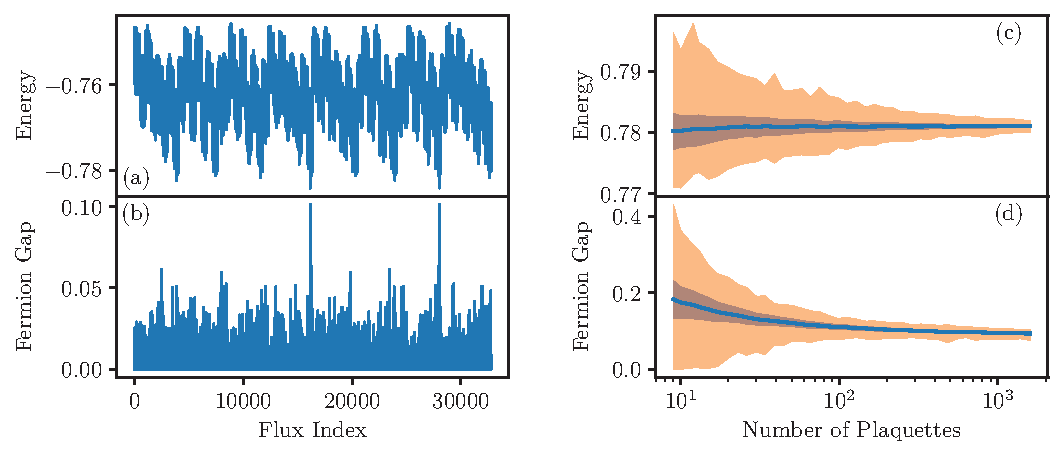
\includegraphics[width=0.9\textwidth]{kitaev_model/figures/ground_state_amorphous.pdf}
    \caption{\textbf{(a)} The energy of every flux sector explored for a system of 16 plaquettes, the order is arbitrary. The two ground state flux sectors can be identified as the points with lowest energy. \textbf{(b)} The fermion gap for each of the flux sectors explored. Note that the largest fermion gap coincides with the ground state flux sector. This occurred in $\sim 85\%$ of cases tested. (c) Average energy of the systems tested over a range of system sizes from $n_p$ = 9 to $n_p = 1600$. The region between the upper and lower quartiles is shown in red, and the full range of energies obtained is shown in orange. (d) Average fermion gap as a function of system size. Again, the region between the upper and lower quartiles is shown in red, and the full range is shown in orange. As can be seen, no gapless systems were found for $n_p > 20$. }
    \label{fig:energy_gaps_example}
\end{figure*}

{\it Testing All Flux Sectors ---}
For a given lattice and flux sector, defined by $\{ u_{jk}\}$, the fermionic ground state energy is calculated by taking the sum of the negative eigenvalues of the matrix
\begin{align}
    M_{jk} = \frac{i}{2} J^{\alpha} u_{jk}.
\end{align}
The set of bond variables $u_{jk}$, which we are free to choose, determine the $\mathbb Z_2$ gauge field. However only the fluxes, defined for each plaquette according to 
\begin{equation}
    \phi_p = \prod_{(j,k) \in \partial p} -iu_{jk},
\end{equation}
have any effect on the energies. Thus, there is enormous degeneracy in the $u_{jk}$ degrees of freedom. Flipping the bonds along any closed loop on the dual lattice has no effect on the fluxes, since each plaquette has had an even number of its constituent bonds flipped - as is shown in the following diagram:
\begin{center}
    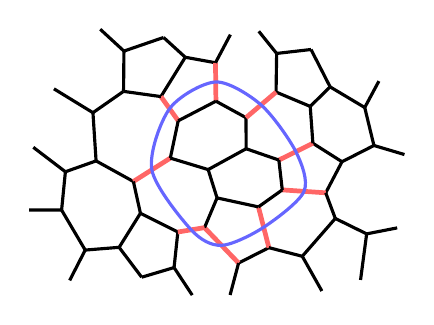
\begin{tikzpicture} 

    \draw [line width=0.4mm,] (2.443089607848154 , 4.199174275000855) --  (2.133663274934363 , 3.699573812024347); 
    \draw [line width=0.4mm,] (2.443089607848154 , 4.199174275000855) --  (2.826766606454033 , 4.129399589956555); 
    \draw [line width=0.6mm,red!60] (2.826766606454033 , 4.129399589956555) --  (2.832350603254511 , 3.6412926004966697); 
    \draw [line width=0.6mm,red!60] (2.133663274934363 , 3.699573812024347) --  (2.3533196431762136 , 3.3923797381398595); 
    \draw [line width=0.4mm,] (2.832350603254511 , 3.6412926004966697) --  (2.3533196431762136 , 3.3923797381398595); 
    \draw [line width=0.4mm,] (2.133663274934363 , 3.699573812024347) --  (1.6590601431591752 , 3.765943303309621); 
    \draw [line width=0.4mm,] (1.7841101988472114 , 2.621425585623738) --  (1.3102001600764661 , 2.8828459026617206); 
    \draw [line width=0.6mm,red!60] (1.7841101988472114 , 2.621425585623738) --  (2.2530706580695927 , 2.918572103800313); 
    \draw [line width=0.4mm,] (1.3102001600764661 , 2.8828459026617206) --  (1.2704284082170167 , 3.4952254145963004); 
    \draw [line width=0.4mm,] (2.2530706580695927 , 2.918572103800313) --  (2.3533196431762136 , 3.3923797381398595); 
    \draw [line width=0.4mm,] (1.6590601431591752 , 3.765943303309621) --  (1.2704284082170167 , 3.4952254145963004); 
    \draw [line width=0.4mm,] (2.832350603254511 , 3.6412926004966697) --  (3.2143675983672417 , 3.4321179123180476); 
    \draw [line width=0.4mm,] (2.7336979624747713 , 2.772672717103165) --  (3.215963942694124 , 3.037305663264089); 
    \draw [line width=0.4mm,] (2.7336979624747713 , 2.772672717103165) --  (2.2530706580695927 , 2.918572103800313); 
    \draw [line width=0.4mm,] (3.215963942694124 , 3.037305663264089) --  (3.2143675983672417 , 3.4321179123180476); 
    \draw [line width=0.4mm,] (1.66412589164998 , 4.27761376616966) --  (1.3628790737427836 , 4.554949458613537); 
    \draw [line width=0.4mm,] (1.66412589164998 , 4.27761376616966) --  (2.1672741059313325 , 4.45048776187154); 
    \draw [line width=0.4mm,] (1.6590601431591752 , 3.765943303309621) --  (1.66412589164998 , 4.27761376616966); 
    \draw [line width=0.4mm,] (1.2704284082170167 , 3.4952254145963004) --  (0.7752117257338569 , 3.7981349822077344); 
    \draw [line width=0.4mm,] (2.443089607848154 , 4.199174275000855) --  (2.1672741059313325 , 4.45048776187154); 
    \draw [line width=0.4mm,] (3.603328735858143 , 4.2476394851768395) --  (3.5960004235960428 , 3.756977430689376); 
    \draw [line width=0.4mm,] (3.603328735858143 , 4.2476394851768395) --  (4.039945897050822 , 4.297661569213179); 
    \draw [line width=0.4mm,] (3.5960004235960428 , 3.756977430689376) --  (4.029745354756155 , 3.5751483526351198); 
    \draw [line width=0.4mm,] (4.029745354756155 , 3.5751483526351198) --  (4.282495230506774 , 3.822901011217539); 
    \draw [line width=0.4mm,] (4.282495230506774 , 3.822901011217539) --  (4.039945897050822 , 4.297661569213179); 
    \draw [line width=0.4mm,] (2.3487551414914605 , 1.9800230663090006) --  (2.300540325954526 , 1.5282907169170128); 
    \draw [line width=0.4mm,] (2.3487551414914605 , 1.9800230663090006) --  (1.8733514017504886 , 2.217815818486644); 
    \draw [line width=0.4mm,] (1.8733514017504886 , 2.217815818486644) --  (1.602858071222523 , 1.785213933169); 
    \draw [line width=0.4mm,] (1.602858071222523 , 1.785213933169) --  (1.8892256504947056 , 1.4056839700867723); 
    \draw [line width=0.4mm,] (2.300540325954526 , 1.5282907169170128) --  (1.8892256504947056 , 1.4056839700867723); 
    \draw [line width=0.4mm,] (4.668899029000971 , 1.370819996056893) --  (4.746438001722542 , 1.956213202683834); 
    \draw [line width=0.4mm,] (4.746438001722542 , 1.956213202683834) --  (4.3482494616334675 , 2.151907119000129); 
    \draw [line width=0.4mm,] (4.3482494616334675 , 2.151907119000129) --  (3.9290282747686036 , 1.6715546842085325); 
    \draw [line width=0.4mm,] (4.177731391775351 , 1.2306194597430695) --  (3.9290282747686036 , 1.6715546842085325); 
    \draw [line width=0.4mm,] (5.1341540722478065 , 2.0322396671565732) --  (4.746438001722542 , 1.956213202683834); 
    \draw [line width=0.4mm,] (3.1199829882043235 , 1.5853535192856314) --  (3.5048132855156084 , 1.7811410414406073); 
    \draw [line width=0.6mm,red!60] (3.1199829882043235 , 1.5853535192856314) --  (2.687310443097729 , 2.0354555882481775); 
    \draw [line width=0.6mm,red!60] (3.5048132855156084 , 1.7811410414406073) --  (3.3721357795131874 , 2.2987943820561982); 
    \draw [line width=0.4mm,] (3.3721357795131874 , 2.2987943820561982) --  (2.8464841372700485 , 2.4130019983886255); 
    \draw [line width=0.4mm,] (2.687310443097729 , 2.0354555882481775) --  (2.8464841372700485 , 2.4130019983886255); 
    \draw [line width=0.6mm,red!60] (2.3487551414914605 , 1.9800230663090006) --  (2.687310443097729 , 2.0354555882481775); 
    \draw [line width=0.4mm,] (3.0121673012212615 , 1.1802036440941053) --  (3.1199829882043235 , 1.5853535192856314); 
    \draw [line width=0.4mm,] (2.5312799405777326 , 1.1785733636646636) --  (2.300540325954526 , 1.5282907169170128); 
    \draw [line width=0.4mm,] (1.8733514017504886 , 2.217815818486644) --  (1.7841101988472114 , 2.621425585623738); 
    \draw [line width=0.4mm,] (2.7336979624747713 , 2.772672717103165) --  (2.8464841372700485 , 2.4130019983886255); 
    \draw [line width=0.4mm,] (4.433307145184742 , 2.872234531196732) --  (4.063679393432637 , 3.1066171115286063); 
    \draw [line width=0.4mm,] (4.433307145184742 , 2.872234531196732) --  (4.226815161490477 , 2.477492472211557); 
    \draw [line width=0.6mm,red!60] (4.226815161490477 , 2.477492472211557) --  (3.674916468623193 , 2.514793378035552); 
    \draw [line width=0.6mm,red!60] (4.063679393432637 , 3.1066171115286063) --  (3.6315308065994065 , 2.893633940528903); 
    \draw [line width=0.4mm,] (3.6315308065994065 , 2.893633940528903) --  (3.674916468623193 , 2.514793378035552); 
    \draw [line width=0.4mm,] (4.83894751221688 , 3.0786317478120138) --  (4.7220696362153936 , 3.5607669867263065); 
    \draw [line width=0.4mm,] (4.83894751221688 , 3.0786317478120138) --  (4.433307145184742 , 2.872234531196732); 
    \draw [line width=0.4mm,] (4.029745354756155 , 3.5751483526351198) --  (4.063679393432637 , 3.1066171115286063); 
    \draw [line width=0.4mm,] (4.7220696362153936 , 3.5607669867263065) --  (4.282495230506774 , 3.822901011217539); 
    \draw [line width=0.4mm,] (4.83894751221688 , 3.0786317478120138) --  (5.226527584560779 , 2.9637036802250862); 
    \draw [line width=0.4mm,] (4.3482494616334675 , 2.151907119000129) --  (4.226815161490477 , 2.477492472211557); 
    \draw [line width=0.4mm,] (3.9290282747686036 , 1.6715546842085325) --  (3.5048132855156084 , 1.7811410414406073); 
    \draw [line width=0.4mm,] (3.3721357795131874 , 2.2987943820561982) --  (3.674916468623193 , 2.514793378035552); 
    \draw [line width=0.4mm,] (3.215963942694124 , 3.037305663264089) --  (3.6315308065994065 , 2.893633940528903); 
    \draw [line width=0.6mm,red!60] (3.2143675983672417 , 3.4321179123180476) --  (3.5960004235960428 , 3.756977430689376); 
    \draw [line width=0.4mm,] (4.7220696362153936 , 3.5607669867263065) --  (4.901832297006263 , 3.8959627247133053); 
    \draw [line width=0.4mm,] (1.3102001600764661 , 2.8828459026617206) --  (0.9205690962626919 , 2.7448693755016778); 
    \draw [line width=0.4mm,] (1.602858071222523 , 1.785213933169) --  (1.1720730675383504 , 1.7504987593424772); 
    \draw [line width=0.4mm,] (0.9205690962626919 , 2.7448693755016778) --  (0.8723030689515361 , 2.258574775850272); 
    \draw [line width=0.4mm,] (0.8723030689515361 , 2.258574775850272) --  (1.1720730675383504 , 1.7504987593424772); 
    \draw [line width=0.4mm,] (2.826766606454033 , 4.129399589956555) --  (3.015687026146436 , 4.486465145140302); 
    \draw [line width=0.4mm,] (3.603328735858143 , 4.2476394851768395) --  (3.376487251015103 , 4.528709024461988); 
    \draw [line width=0.4mm,] (0.9205690962626919 , 2.7448693755016778) --  (0.5128878465410877 , 3.0556589636233125); 
    \draw [line width=0.4mm,] (0.8723030689515361 , 2.258574775850272) --  (0.46147593859581926 , 2.2588828762828306); 
    \draw [line width=0.4mm,] (1.1720730675383504 , 1.7504987593424772) --  (0.9748432903949585 , 1.3652738897280694); 
    \draw [blue!60,line width=0.4mm] plot [smooth cycle] coordinates { (2.0185904284584018, 2.769998844712026)  (2.2434914590552886, 3.5459767750821034)  (2.829558604854272, 3.8853460952266126)  (3.405184010981642, 3.5945476715037117)  (3.8476051000160214, 3.0001255260287545)  (3.950865815056835, 2.4961429251235545)  (3.438474532514398, 2.0399677117484027)  (2.903646715651026, 1.8104045537669045)  (2.5180327922945946, 2.007739327278589) };
    
    \end{tikzpicture}
\end{center}
where the flipped bonds are shown in red. In order to explore every possible flux sector using the $u_{jk}$ variables, we restrict ourselves to change only a subset of the bonds in the system. In particular, we construct a spanning tree on the dual lattice, which passes through every plaquette in the system, but contains no loops. 
\begin{center}
    \input{kitaev_model/figures/tikzpictures/spanning_tree.tex}
\end{center}
The tree contains $n_p - 1$ edges, shown in red, whose configuration space has a $1:1$ mapping onto the $2^{n_p - 1}$ distinct flux sectors. Each flux sector can be created in precisely one way by flipping edges only on the tree (provided all other bond variables not on the tree remain fixed). Thus, all possible flux sectors can be accessed by iterating over all configurations of edges on this spanning tree.

{\it Finite Size Effects ---}
In our numerical investigation, the objective was to test as many example lattices as possible. We aim for the largest lattice size that could be efficiently solved, requiring a balance between lattice size and cases tested. Each added plaquette doubles the number of flux sectors that must be checked. 25,000 lattices containing 16 plaquettes were used. However, in his numerical investigation of the honeycomb model, Kitaev demonstrated that finite size effects persist up to much larger lattice sizes than we were able to access \cite{kitaev_anyons_2006}. \par 
In order to circumvent this problem, we treat the 16-plaquette amorphous lattice as a unit cell in an arbitrarily large periodic system. The bonds that originally connected across the periodic boundaries now connect adjacent unit cells. This infinite periodic Hamiltonian can then be solved using Bloch's theorem, since the larger system is diagonalised by a plane wave ansatz. For a given crystal momentum $\bf q \in [0,2\pi)^2 $, we are left with a Bloch Hamiltonian, which is identical to the original Hamiltonian aside from an extra phase on edges that cross the periodic boundaries in the $x$ and $y$ directions,
\begin{align}
    M_{jk}(\bf q) =  \frac{i}{2} J^{\alpha} u_{jk} e^{i q_{jk}},
\end{align}
where $q_{jk} = q_x$ for a bond that crosses the $x$-periodic boundary in the positive direction, with the analogous definition for $y$-crossing bonds. We also have $q_{jk} = -q_{kj}$. Finally $q_{jk} = 0$ if the edge does not cross any boundaries at all -- in essence we are imposing twisted boundary conditions on our system. The total energy of the tiled system can be calculated by summing the energy of $M(\bf q)$ for every value of $\bf q$. In practice we constructed a lattice of $50 \times 50$ values of $\bf q$ spanning the Brillouin zone. The procedure is called twist averaging because the energy-per-unit cell is equivalent to the average energy over the full range of twisted boundary conditions. \par 
{\it Evidence for the Ground State Ansatz ---}
For each lattice with 16 plaquettes, $2^{15} =$ 32,768 flux sectors are generated. In each case we find the energy (averaged over all twist values) and the size of the fermion gap, which is defined as the lowest energy excitation for any value of $\bf q$. We then check if the lowest energy flux sector aligns with our ansatz (given by $\phi^{\textup{g.s.}}_p = -(\pm i)^{n_{\textup{sides}}}$) and whether this flux sector is gapped. \par
In the isotropic case ($J^\alpha = 1$), all 25,000 examples conformed to our guess for the ground state flux sector. A tiny minority ($\sim 10$) of the systems were found to be gapless. As we shall see shortly, the proportion of gapless systems vanishes as we increase the size of the amorphous lattice. An example of the energies and gaps for one of the systems tested is shown in fig.~\ref{fig:energy_gaps_example} (a). For the anisotropic phase (we used $ J^x, J^y = 0.25, J^z = 1$) the overwhelming majority of cases adhered to our ansatz, however a small minority ($\sim 0.5 \%$) did not. In these cases, however, the energy difference between our ansatz and the ground state was at most of order $10^{-6}$. Further investigation would need to be undertaken to determine whether these anomalous systems are a finite size effect due to the small amorphous system sizes used or a genuine feature of the toric code phase on such lattices. \par

{\it A Gapped Ground State ---} Now that we have collected sufficient evidence to support our guess for the ground state flux sector, we turn our attention to checking that this sector is gapped. We no longer need to exhaustively search over flux space for the ground state, so it is possible to go to much larger system size. We generate 40 sets of systems with plaquette numbers ranging from 9 to 1600. For each system size, 1000 distinct lattices are generated and the energy and gap size are calculated without phase twisting, since the effect is negligible for such large system sizes. As can be seen in fig.~\ref{fig:energy_gaps_example} (c-d), for very small system size a small minority of gapless systems appear, however beyond around 20 plaquettes all systems had a stable fermion gap in the ground state. Finally, the energy and gap difference between the phase twisted and non-phase twisted results vanished exponentially with the system size, supporting the claim that the results can be straightforwardly extrapolated to large systems. 

\subsection{Time Reversal Symmetry}

\subsection{The Ground-State Phase Diagram}